\documentclass{article}      % Specifies the document class

\usepackage[margin=1.5in]{geometry}
\usepackage{listings}
\usepackage{tikz}
\usetikzlibrary{calc}
\usetikzlibrary{shapes,arrows}

\title{Bitflate: A Cryptocurrency with Constant Inflation}
\author{The Bitflate Community \\ contact@bitflate.org \\ bitflate.org}
\date{February 2021}

\begin{document}             % End of preamble and beginning of text.

\maketitle                   % Produces the title.

\begin{abstract}
Bitcoin is a groundbreaking invention. It pioneered a new form of digital native money. It overcame the challenges that failed previous attempts. In the Bitcoin whitepaper, Satoshi Nakamoto presented Bitcoin as an electronic cash system. However, it has evolved into digital gold. The search for digital cash remains elusive. It is a contentious issue in the Bitcoin community. Bitcoin with a block size of 1MB, originally coded by Satoshi Nakamoto, is more suitable to be digital gold. The big-block hard fork, Bitcoin Cash, has not proved to be the answer for digital cash. In this paper, we present Bitflate, a cryptocurrency with constant inflation. We believe Biflate is a component of digital cash. What humans perceive as money is a fluid concept. Money changes over time. It cannot be defined precisely. We present an elastic money system built on top of Bitcoin and Bitflate. This elasticity allows us to create hybrid currencies. These hybrid currencies can be used as digital cash.
\end{abstract}

\section{Background}
Humans discovered gold more than 40,000 years ago. The shiny metal has been used as money since at least 5,000 years ago. Paper money was invented in the 7th century. The Gold Standard continued to be the base money. Gold can bring long-term price stability. But in the short-term, it can be volatile, especially during an economic crisis [1]. Gold's supply is limited. It has a stock-to-flow ratio of 60. That means its supply doubles every 60 years. This stock-to-flow ratio translates roughly to a 1.2\% inflation rate [7]. Gold served as a standard instrument to measure progress across economies. Without a standard, it is hard to assess values. As human civilization progresses, money has evolved to include three functions:

\begin{itemize}
   \item A Store of Value: This property allows people to retain the purchasing power of their money.

   \item A Medium of Exchange: This property encourages people to spend. Consumption facilitates commerce and economic development.

   \item A Unit of Account: This property allows people to assess values across different goods and assets.
\end{itemize}

These functions are necessary to facilitate economic development. But sometimes, they are conflicting with each other. For example, if money is used as a Store of Value, people will be hoarding it. They are hesitant to use it for spending. It does not work well as a Medium of Exchange. Gold is an example of this form of money. Given its low supply inflation, people often use it as a Store of Value. Gold is scarce but ubiquitous. People and cultures are familiar with it. So it was used as a Medium of Exchange and a Unit of Account. Gold was the de facto money throughout history. The Gold Standard tried to fit three money functions into gold. This standard showed problems during economic crises like the Great Depression. Because of scarcity, governments were unable to stimulate economic development. The lack of stimulus prolongs recession.

With improved technology and communication, the world has moved to the US Dollar system. Under this system, the US Dollar is the reserve currency. It is managed by the Federal Reserve. It is the Medium of Exchange and Unit of Account for commerce. It also serves as a Store of Value for countries without stable currencies. The US Dollar has replaced gold. It performs the three functions of money. After a few decades, the US Dollar system began to show problems. Its dual functions as a Store of Value and a Medium of Exchange are conflicting. They create a trade imbalance between the US and other countries. As the world demands more dollars, economies flood the US with goods to access the reserve currency. Manufacturing has become cheaper outside the US. Outsourcing, technology, and automation increase wealth inequality and political turmoil.

In 2008, Satoshi Nakamoto, an anonymous programmer, released Bitcoin. It uses a peer-to-peer network of computers to enable decentralization. Bitcoin has no central authority. Each node can verify transactions and balances. Bitcoin's monetary policy resembles gold. It is scarce. The eventual supply of bitcoins is 21 million. After the third halving in May 2020, Bitcoin's supply increases at 1.79\% per year [2]. The rate will continue to decrease until 2140. At that point, the block reward will be 0. Bitcoin's supply will stop increasing. Scarcity makes Bitcoin a deflationary and valuable asset. By early 2021, Bitcoin's market capitalization has grown to 1 trillion dollars. Bitcoin's supporters laud it as the final form of money. It will enable the Bitcoin Standard. Money will be pegged to Bitcoin. The Bitcoin Standard is similar to the Gold Standard. Bitcoin will perform the three functions of money: a Store of Value, a Medium of Exchange, and a Unit of Account. Like gold, this system has shown similar problems. Bitcoin's price has been volatile. Because Bitcoin is scarce, users prefer to hold. Its usage as payment has not gained adoption. It is probably impossible to reconcile three functions of money into one monetary system. The Gold Standard and the Dollar are examples. During an economic crisis, the functions will conflict with each other.

\section{Motivation \& Design}

Bitcoin is an important breakthrough [4]. It has successfully created digital gold, a new Store of Value. But it is futile to fit other money functions into one deflationary monetary policy. The Gold Standard and the US Dollar system were not flexible to perform all three functions. Fortunately, Bitcoin is a digital system. We can expand the system to accommodate new scenarios. Teams have created forks to address the payment scenario. Bitcoin Cash is a hard fork to increase block size. A larger block size can accommodate more transactions. But volatility is an inherent property of Bitcoin's supply. More transactions do not reduce price volatility.

To prevent hoarding, another approach is demurrage [6]. Freicoin is a demurrage currency [5]. Demurrage and inflation are different. Demurrage imposes tax at the individual level. It requires individual actions. Inflation imposes tax at the group level. It requires no individual actions, but group actions. Demurrage requires people to make a choice: spending or not spending and get taxed. Demurrage makes more sense from the view of individualism. Inflation makes more sense from the view of collectivism.

We have identified inflation as the key to unlock the transaction use case. Inflation discourages hoarding. It encourages people to spend. Some have proposed a dynamically adjusted inflation rate. Supply responds to price demand. This design relies on external information. Nodes have to query exchanges for price information. A constant inflation rate adheres to the same principles of Bitcoin. The system can be decentralized and free of monetary manipulation.

We have designed and implemented Bitflate, a cryptocurrency with 7\% supply inflation. Bitflate is a software fork of Bitcoin. We want to introduce inflation and retain the decentralization properties. We picked 7\% per year as the inflation rate. With a 7\% inflation rate, Bitflate's supply doubles about every 10 years (Rule of 72 [3]). Bitflate's most prominent feature is inflation. If it has a low rate of 1\%, it would behave like a Store of Value. If the inflation rate is too high, people don't have incentives to hold Bitflate coins. Hyperinflation can be volatile. A high rate can hinder the adoption of the system. A moderately high rate strikes the balance. It will allow us to build a more flexible monetary system.

To bootstrap Bitflate, the system gives more block rewards to early adopters. The rewards halve 3 times before 7\% inflation starts. The table in Figure 1 shows block reward for the first 10 eras.

\begin{figure}[h]
\centering
\begin{tabular}{ |c|l| } 
 \hline
 era & reward \\
 \hline
 0  & 50 \\
 1 & 25 \\
 2 & 12.5 \\
 3 & 6.25 (end of halving) \\
 4 & 6.56 (7\% inflation) \\
 5 & 7.02 \\
 6 & 7.51 \\
 7 & 8.04 \\
 8 & 8.60 \\
 9 & 9.20 \\
 10 & 9.85 \\
 \hline
\end{tabular}
\caption{Bitflate Block Reward}
\end{figure}

At a 7\% growth rate, Bitflate's supply will reach 31 million in 10 years, 122 million in 30 years, and 14 billion in 100 years. This is an exponential growth rate. Some altcoins, like Grin, Dogecoin, have unlimited supply. But they have a constant tail emission. Their supply curves are asymptotic. Growth rates decrease and approach 0. With an inflationary supply, Bitflate does not have the fair distribution problem like other altcoins. Inflation encourages people to spend their Bitflate coins.

\section{Software}

Bitflate Core is a software fork of Bitcoin Core. We intend to keep Bitflate updated with the Bitcoin technology stack. The table in Figure 2 shows the prominent differences between the Bitflate Core software and the Bitcoin Core software.

\begin{figure}[h]
\centering
\begin{tabular}{ |l|l|l| } 
 \hline
 Feature & Bitflate & Bitcoin \\
 \hline
 Reward & Inflationary 7\% per year & Deflationary \\
 \hline
 Supply & Unlimited & 21 million \\
 \hline
 Block time & 2.5 minutes & 10 minutes \\
 \hline
 Reward change & Every 210,000 blocks (1 year) & Every 210,000 blocks (4 years) \\
 \hline
 Proof of Work Target & 3.5 days & 14 days \\
 \hline
 Port & 7333 & 8333 \\
 \hline
\end{tabular}
\caption{Differences between the Bitflate and Bitcoin software}
\end{figure}

The most important code change in the Bitflate software is the block subsidy calculation. The code is below.

\begin{lstlisting}[language=C++]
CAmount GetBlockSubsidy(int nHeight, const Consensus::Params& consensusParams)
{
  int halvings = nHeight / consensusParams.nSubsidyHalvingInterval;
  CAmount nSubsidy = 0;
  // Inflation starts at halving 4.
  // At that point, we'd have 19,687,500 (~ 19 million) coins.
  // Those are our base coins.
  // See bitcoin supply schedule
  // After halving 3, we calculate the inflate coin number.
  if (halvings > 3) {
    // calculate coin inflation for this halving
    CAmount inflateCoins =
      round(19687500 * (pow(1.07, halvings - 3) - pow(1.07, halvings - 4)));
    // subsidy is inflateCoins / 210000 * COIN
    nSubsidy = ((int)round((inflateCoins / 210000.0) * 100)) * (COIN / 100);
  } else {
    nSubsidy = 50 * COIN;
    // Subsidy is cut in half every 210,000 blocks
    // which will occur approximately every 4 years.
    nSubsidy >>= halvings;
  }
  return nSubsidy;
}
\end{lstlisting}

Bitflate has the same block size as Bitcoin with SegWit enabled. With a smaller block time of 2.5 minutes, the Bitflate network produces blocks 4 times faster than the Bitcoin network. This change increases the transaction throughput. But it is not a significant improvement. It is not exponential scaling. We expect Bitflate will need off-chain scaling for transactions.

\section{Elastic Monetary System}

A monetary system comes with tradeoffs. If it is scarce, it is more like a Store of Value. Scarcity prevents it from being a Medium of Exchange. Crypto money systems are programmable and more flexible. We can design a system to accommodate all three functions of money. We present an elastic monetary system built on top of Bitcoin and Bitflate. The base blockchains are the anchors of the system. Bitcoin is the Store of Value anchor. Bitflate is the Medium of Exchange anchor.

By mixing Bitcoin and Bitflate, we can create hybrid cryptocurrencies that have inflation rates between 0\% and 7\%. For example, in 2030, a financial provider wants to issue a coin that inflates at 3\% per year. Let's call this coin Bit3. For simplicity, let's assume the Bitcoin supply is 21 million. It no longer inflates. Bitflate supply is 30 million. It inflates at 7\% per year. In 2031, Bitflate supply will reach 33 million. At the time of this Bit3 issuance, 1 Bitcoin is equivalent to 1.4 Bitflate (30 million/21 million). If we mix ratio 1/1.4, we'd get a coin that has a supply inflation of 3.5\%. To lower the inflation rate, we need to mix fewer Bitflate coins. In this case, the mix ratio is 1 Bitcoin and 1.2 Bitflate. This mixed cryptocurrency has a supply inflation of 3\% per year.

If a hybrid cryptocurrency has more Bitcoin than Bitflate, it retains more value over time. It is more volatile. If a hybrid cryptocurrency has more Bitflate than Bitcoin, it devalues over time. Its value is more stable. It is more suitable for transactions. If a central bank wants to target 2\% inflation, they can peg their fiat currency with a 2\% hybrid cryptocurrency. The fiat currency can continue to be used as the Unit of Account. It is exchangeable for the underlying Bitcoin and Bitflate. During an economic crisis, the central bank can devalue their fiat currency by moving the peg higher. This elastic money system is flexible and transparent. It is decentralized. It allows the free market to generate and price currencies. Digital cash is not a coin. It is an amalgamation of coins with different money properties.

\begin{figure}[h]
\centering
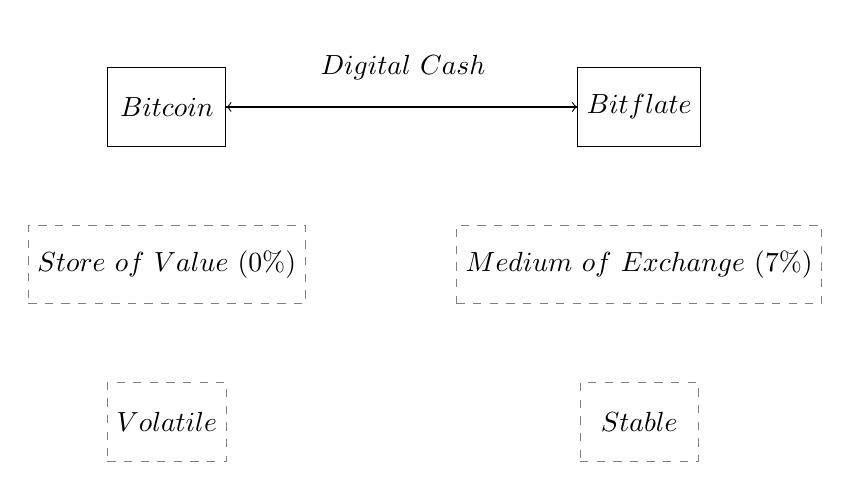
\begin{tikzpicture}[
    squarednode/.style={rectangle, draw=gray,dashed},
    textnode/.style={rectangle, draw=white,dashed},
    emptytextnode/.style={rectangle, text=white, draw=white,dashed}
    ]
  \begin{scope}[minimum width=15mm,minimum height=10mm]
    % nodes
    \node[emptytextnode] (Empty) at (0,0) {$Empty$};
    \node[draw] (Bitcoin) at ($(Empty)+(0,-0.5)$) {$Bitcoin$};
    \node[draw] (Bitflate) at ($(Bitcoin)+(6,0)$) {$Bitflate$};
    \node[squarednode] (Store of Value) at ($(Bitcoin)+(0,-2)$) {$Store\ of\ Value\ (0\%)$};
    \node[squarednode] (Medium of Exchange) at ($(Bitcoin)!1!(Bitflate)+(0,-2)$) {$Medium\ of\ Exchange\ (7\%)$};
    \node[squarednode] (Volatile) at ($(Bitcoin)+(0,-4)$) {$Volatile$};
    \node[squarednode] (Stable) at ($(Bitcoin)!1!(Bitflate)+(0,-4)$) {$Stable$};
    \node[textnode] at ($(Bitcoin)+(3,0.5)$) {$Digital\ Cash$};
    % arrows
    \draw [->] (Bitcoin) -- (Bitflate);
    \draw [->] (Bitflate) -- (Bitcoin);
  \end{scope}
  % arrows
    
\end{tikzpicture}
\caption{Elastic Monetary System}
\end{figure}

\section{Conclusion}

We discussed the history of monetary systems based on gold and the US dollar. Bitcoin creates a new form of digital money. However, its deflationary supply has the same problem with volatility as gold. Bitcoin, by itself, cannot fulfill all three functions of money: a Store of Value, a Medium of Exchange, and a Unit of Account.

We have proposed Bitflate, an inflationary cryptocurrency and an elastic monetary system. This elastic monetary system is flexible and transparent. It allows the free market to create hybrid currencies. They are redeemable into Bitcoin and Bitflate. The base coins can be remixed to serve a new function.

\begin{thebibliography}{9}

\bibitem{goldstandard} 
Gold Standard Disadvantages
\\\texttt{$https://en.wikipedia.org/wiki/Gold_standard\#Disadvantages$}

\bibitem{bitcoinsupply} 
Bitcoin's Supply
\\\texttt{$https://en.bitcoin.it/wiki/Controlled_supply$}

\bibitem{rule72} 
Rule of 72
\\\texttt{$https://en.wikipedia.org/wiki/Rule_of_72$}

\bibitem{bitcoinwhitepaper} 
The Bitcoin Whitepaper
\\\texttt{$https://bitcoin.org/bitcoin.pdf$}

\bibitem{freicoin}
Freicoin
\\\texttt{$http://freico.in/$}

\bibitem{demurrage}
Demurrage (currency)
\\\texttt{$https://en.wikipedia.org/wiki/Demurrage_(currency)$}

\bibitem{golds2f}
Gold's Stock-To-Flow Ratio And Why It Matters
\\\texttt{$https://seekingalpha.com/article/4357409-golds-stock-to-flow-ratio-and-why-matters$}

\end{thebibliography}

\begin{appendix}
\section{Source Code}

https://github.com/bitflate/bitflate

\section{Bitflate Supply for 100 Eras (Years)}

Spreadsheet: {$https://docs.google.com/spreadsheets/d/1tdRWdqc0I9uMASXp-zY8TnVhoiTJUd-NIEnQrAl_3Lg/edit?usp=sharing$}

\begin{center}
\begin{tabular}{ |c|r|r|r|r| } 
 \hline
 Era & Reward & Issued Coins & Total Coins & Supply Increase Rate \\
 \hline
 0  & 50 & 10500000 & 10500000 & N/A \\
 1 & 25 & 5250000 & 15750000 & 50 \\
 2 & 12.5 & 2625000 & 18375000 & 16.66666667 \\
 3 & (end of halving) 6.25 & 1312500 & 19687500 & 7.142857143 \\
 4 & (7\% inflation) 6.56 & 1378125 & 21065100 & 6.997333333 \\
 5 & 7.02 & 1474594 & 22539300 & 6.998305254 \\
 6 & 7.51 & 1577815 & 24116400 & 6.997111712 \\
 7 & 8.04 & 1688262 & 25804800 & 7.001044932 \\
 8 & 8.60 & 1806441 & 27610800 & 6.998697917 \\
 9 & 9.20 & 1932892 & 29542800 & 6.997261941 \\
 10 & 9.85 & 2068194 & 31611300 & 7.001705999 \\
 11 & 10.54 & 2212968 & 33824700 & 7.001926526 \\
 12 & 11.28 & 2367875 & 36193500 & 7.003166325 \\
 13 & 12.06 & 2533627 & 38726100 & 6.997389034 \\
 14 & 12.91 & 2710980 & 41437200 & 7.000704951 \\
 15 & 13.81 & 2900749 & 44337300 & 6.998783702 \\
 16 & 14.78 & 3103802 & 47441100 & 7.000426278 \\
 17 & 15.81 & 3321068 & 50761200 & 6.99836218 \\
 18 & 16.92 & 3553542 & 54314400 & 6.999834519 \\
 19 & 18.11 & 3802290 & 58117500 & 7.002010517 \\
 20 & 19.37 & 4068451 & 62185200 & 6.999096658 \\
 21 & 20.73 & 4353242 & 66538500 & 7.000540321 \\
 22 & 22.18 & 4657969 & 71196300 & 7.000157803 \\
 23 & 23.73 & 4984027 & 76179600 & 6.999380586 \\
 24 & 25.39 & 5332909 & 81511500 & 6.999117874 \\
 25 & 27.17 & 5706213 & 87217200 & 6.999871184 \\
 26 & 29.07 & 6105647 & 93321900 & 6.999422132 \\
 27 & 31.11 & 6533043 & 99855000 & 7.000607574 \\
 28 & 33.29 & 6990356 & 106845900 & 7.001051525 \\
 29 & 35.62 & 7479681 & 114326100 & 7.00092376 \\
 30 & 38.11 & 8003258 & 122329200 & 7.000238791 \\
 31 & 40.78 & 8563486 & 130893000 & 7.000618005 \\
 32 & 43.63 & 9162930 & 140055300 & 6.999839564 \\
 33 & 46.69 & 9804335 & 149860200 & 7.00073471 \\
 34 & 49.96 & 10490639 & 160351800 & 7.000924862 \\
 35 & 53.45 & 11224984 & 171576300 & 6.999921423 \\
 36 & 57.19 & 12010733 & 183586200 & 6.999742971 \\
 37 & 61.2 & 12851484 & 196438200 & 7.000526183 \\
 38 & 65.48 & 13751088 & 210189000 & 7.000064142 \\
 39 & 70.07 & 14713664 & 224903700 & 7.000699371 \\
 40 & 74.97 & 15743620 & 240647400 & 7.000196084 \\
 41 & 80.22 & 16845674 & 257493600 & 7.000366511 \\
 42 & 85.83 & 18024871 & 275517900 & 6.999902133 \\
 43 & 91.84 & 19286612 & 294804300 & 7.000053354 \\
 44 & 98.27 & 20636675 & 315441000 & 7.000135344 \\
 45 & 105.15 & 22081242 & 337522500 & 7.00019972 \\
 46 & 112.51 & 23626929 & 361149600 & 7.000155545 \\
 47 & 120.38 & 25280814 & 386429400 & 6.999813928 \\
 48 & 128.81 & 27050471 & 413479500 & 7.000010869 \\
 49 & 137.83 & 28944004 & 442423800 & 7.00017776 \\
 50 & 147.48 & 30970084 & 473394600 & 7.000256315 \\
 \hline
\end{tabular}
\end{center}

\begin{center}
\begin{tabular}{ |c|r|r|r|r| } 
 \hline
 Era & Reward & Issued Coins & Total Coins & Supply Increase Rate \\
 \hline
 51 & 157.8 & 33137990 & 506532600 & 7.000079849 \\
 52 & 168.85 & 35457649 & 541991100 & 7.000240458 \\
 53 & 180.67 & 37939685 & 579931800 & 7.0002441 \\
 54 & 193.31 & 40595463 & 620526900 & 6.999978273 \\
 55 & 206.84 & 43437145 & 663963300 & 6.999922163 \\
 56 & 221.32 & 46477745 & 710440500 & 6.999965209 \\
 57 & 236.82 & 49731187 & 760172700 & 7.000192134 \\
 58 & 253.39 & 53212370 & 813384600 & 6.999975137 \\
 59 & 271.13 & 56937236 & 870321900 & 7.000046472 \\
 60 & 290.11 & 60922843 & 931245000 & 7.000065148 \\
 61 & 310.42 & 65187442 & 996433200 & 7.000112752 \\
 62 & 332.15 & 69750563 & 1066184700 & 7.000118021 \\
 63 & 355.4 & 74633102 & 1140818700 & 7.000100452 \\
 64 & 380.27 & 79857419 & 1220675400 & 6.999946617 \\
 65 & 406.89 & 85447439 & 1306122300 & 6.999969034 \\
 66 & 435.38 & 91428760 & 1397552100 & 7.000094861 \\
 67 & 465.85 & 97828773 & 1495380600 & 6.999989482 \\
 68 & 498.46 & 104676787 & 1600057200 & 6.999997191 \\
 69 & 533.35 & 112004162 & 1712060700 & 6.999968501 \\
 70 & 570.69 & 119844453 & 1831905600 & 7.000038024 \\
 71 & 610.64 & 128233565 & 1960140000 & 7.000055025 \\
 72 & 653.38 & 137209915 & 2097349800 & 7 \\
 73 & 699.12 & 146814609 & 2244165000 & 7.000034043 \\
 74 & 748.06 & 157091631 & 2401257600 & 7.000046788 \\
 75 & 800.42 & 168088045 & 2569345800 & 7.000006996 \\
 76 & 856.45 & 179854208 & 2749200300 & 7.000011443 \\
 77 & 916.4 & 192444003 & 2941644300 & 6.999999236 \\
 78 & 980.55 & 205915083 & 3147559800 & 7.000013564 \\
 79 & 1049.19 & 220329139 & 3367889700 & 7.000022684 \\
 80 & 1122.63 & 235752179 & 3603642000 & 7.000000624 \\
 81 & 1201.21 & 252254831 & 3855896100 & 6.99997669 \\
 82 & 1285.3 & 269912670 & 4125809100 & 7.00000708 \\
 83 & 1375.27 & 288806556 & 4414615800 & 7.000001527 \\
 84 & 1471.54 & 309023015 & 4723639200 & 7.00000666 \\
 85 & 1574.55 & 330654626 & 5054294700 & 7.000016005 \\
 86 & 1684.76 & 353800450 & 5408094300 & 6.999979641 \\
 87 & 1802.7 & 378566482 & 5786661300 & 7.000007378 \\
 88 & 1928.89 & 405066136 & 6191728200 & 7.000010524 \\
 89 & 2063.91 & 433420765 & 6625149300 & 7.000002035 \\
 90 & 2208.38 & 463760219 & 7088909100 & 6.999990174 \\
 91 & 2362.97 & 496223434 & 7585132800 & 7.000000889 \\
 92 & 2528.38 & 530959074 & 8116092600 & 7.000006645 \\
 93 & 2705.36 & 568126209 & 8684218200 & 6.999989133 \\
 94 & 2894.74 & 607895044 & 9292113600 & 7.000001451 \\
 95 & 3097.37 & 650447697 & 9942561300 & 6.999997288 \\
 96 & 3314.19 & 695979036 & 10638541200 & 7.000006125 \\
 97 & 3546.18 & 744697569 & 11383239000 & 6.99999921 \\
 98 & 3794.41 & 796826398 & 12180065100 & 6.999994466 \\
 99 & 4060.02 & 852604246 & 13032669300 & 6.999997069 \\
 100 & 4344.22 & 912286543 & 13944955500 & 6.999995005 \\
 101 & 4648.32 & 976146602 & 14921102700 & 7.000002259 \\
 \hline
\end{tabular}
\end{center}

\end{appendix}

\end{document}               % End of document.